%
% This docuement is based on the Insight Journal Template.
% https://github.com/InsightSoftwareConsortium/InsightJournalTemplate/tree/ModularTemplate
% 4555fc04b105b11f06dc302b76bf09c27e50727d

\documentclass{InsightArticle}

\usepackage[dvips]{graphicx}
%  hyperref should be the last package to be loaded.
\usepackage[dvips,
bookmarks,
bookmarksopen,
float,
backref,
colorlinks,linkcolor={blue},citecolor={blue},urlcolor={blue},
]{hyperref}

\title{BinShrink: A multi-resolution filter with cache efficient averaging. }

\newcommand{\IJhandlerIDnumber}{0}

\release{0.00}

% At minimum, give your name and an email address.  You can include a
% snail-mail address if you like.
\author{Bradley C. Lowekamp$^{1}$ and David T. Chen$^{1}$}
\authoraddress{$^{1}$National Library Of Medicine}

\begin{document}

%
% Add hyperlink to the web location and license of the paper.
% The argument of this command is the handler identifier given
% by the Insight Journal to this paper.
% 
\IJhandlefooter{\IJhandlerIDnumber}


\ifpdf
\else
   %
   % Commands for including Graphics when using latex
   % 
   \DeclareGraphicsExtensions{.eps,.jpg,.gif,.tiff,.bmp,.png}
   \DeclareGraphicsRule{.jpg}{eps}{.jpg.bb}{`convert #1 eps:-}
   \DeclareGraphicsRule{.gif}{eps}{.gif.bb}{`convert #1 eps:-}
   \DeclareGraphicsRule{.tiff}{eps}{.tiff.bb}{`convert #1 eps:-}
   \DeclareGraphicsRule{.bmp}{eps}{.bmp.bb}{`convert #1 eps:-}
   \DeclareGraphicsRule{.png}{eps}{.png.bb}{`convert #1 eps:-}
\fi


\maketitle


\ifhtml
\chapter*{Front Matter\label{front}}
\fi

% The abstract should be a paragraph or two long, and describe the
% scope of the document.
\begin{abstract}
\noindent
We present a new filter for the Insight Toolkit (ITK) for reducing the
resolution of an image by an integer factor while averaging called
\textit{BinShrink}. This filter provides a new level of performance to
ITK for reducing resolution and noise present in an image. The filter
supports streaming, multi-threading and most of ITK's pixel types
including scalars, \textit{Vector}s,
\textit{SymmetricSecondRankTensor}s, and \textit{RGBPixel}s.

\end{abstract}

\IJhandlenote{\IJhandlerIDnumber}

\tableofcontents

Using filters from the Insight Toolkit, we develop an algorithm for detecting
and tracking thje movement of solar spots. As it is widely known, celestial
objects such as the sun are ethereal and perfect, and therefore can not harbor
artifacts such as spots. However, observations performed with our open source
telescope have revealed the presence of such spots. The spots seems to continuously change positions on the solar surface. 


% don't like
This ``binning'' algorithm is commonly used in processing of high
resolution electron microscopy image. It's available in such packages
as The Boulder Laboratory for 3-D Electron Microscopy of Cell's
IMOD\cite{IMOD}, \cite{bsoft2007}. 
Multi-resolution

Why is this filter useful?


This document describes a new algorithm not currently in
ITK\cite{ITKSoftwareGuide}. 

\section{Implementation}

Algorithm

Features

\subsection{Geometry}


\begin{figure}
  \centering
  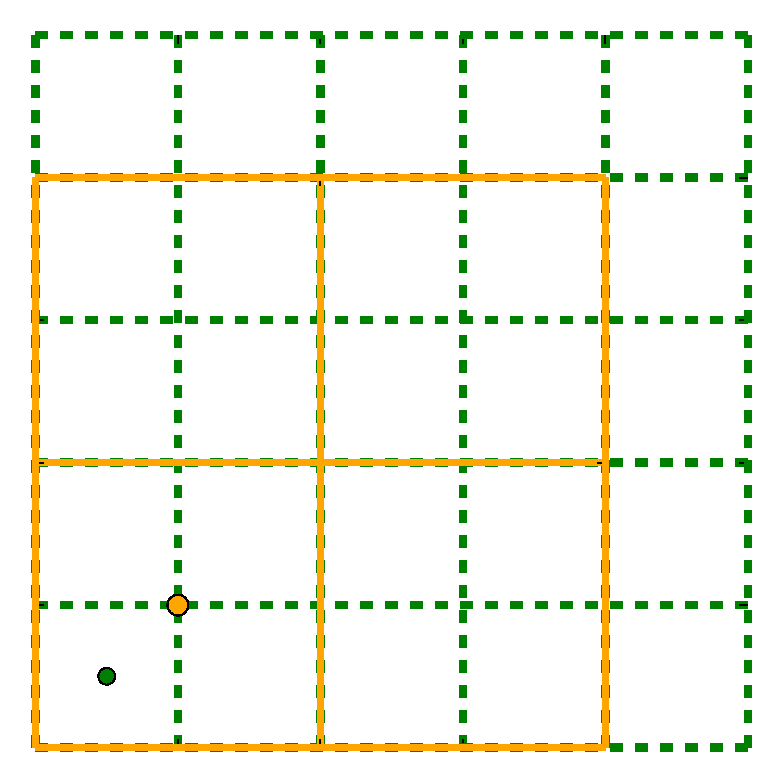
\includegraphics[width=0.8\linewidth]{images/pixelgrid}
  \itkcaption{Grid Geometry}
  \label{fig:PixelGrid}
\end{figure}

\subsection{Optimization}
Optimization 


\section{Results}

To test our BinShrink filter we have used a synthetic function
created by Marschner and Lobb\cite{MarschnerL94}, along with additive
noise to create test volume images. This function is often used to
evaluate volume rendering reconstruction filters. We have rendered it
into a 128 pixel cubic volume such that the majority of the frequencies in
the function are sampled just above 4 times the Nyquist frequency. Such an image
makes for a challenging theoretical data set when the shrinking factor is also
4.

The code used to generate these images was written in Python with
SimpleITK. The original Marshner-Lobb volume was normalized with the 
\textit{Normalize} filter so that the volume had a mean
of 0 and a standard deviation of 1. Then Gaussian distributed random
noise was added with a 0 mean and a sigma to achieve the targeted
signal to noise ratio. After the shrinking operation was performed,
the volume was again normalized for contrast. Then the center slice
was extracted and tiled. Finally it was colorized by the
\textit{ScalarToRGBColormap} filter\cite{Tustison2009}.

We examined the results of the \textit{BinShrink} filter by varying the
signal to noise ratio in our Marshnel-Lobb test image and then shrinking those noisy
images by factors of 2 and 4 (See figure
\ref{fig:BinShrinkComparison}). For comparison we also used the
\textit{SmoothingRecusiveGaissian} filter in conjunction with the
\textit{Shrink} filter on the same test noisy images.  We set \textit{sigma} of the
smoothing Gaussian kernel at 0.7 times the shrink factor. 

[NEED TO TALK ABOUT ALIASING AND IMAGE QUALITY, SINCE IT'S MENTIONED IN THE CONCLUSION]

\begin{figure}
  \centering
  \includegraphics[width=0.4\linewidth]{images/binshrink_hot.png}
  \caption[Registration Framework Components]{The basic components of the
    registration framework are two input images, a transform, a metric, an
    interpolator and an optimizer.}
  \label{fig:BinShrinkComparison}
\end{figure}

\begin{figure}
  \centering
  \includegraphics[width=0.4\linewidth]{images/gaussianshrink_hot.png}
  \caption[Registration Framework Components]{The basic components of the
    registration framework are two input images, a transform, a metric, an
    interpolator and an optimizer.}
  \label{fig:GaussianShrinkComparison}
\end{figure}

\subsection{Performance}

To analyze the performance of our bin shrinking methods we compare them
against similar processes which can be performed in ITK with other pairs of filters.

Running a \textit{Mean} filter followed by a \textit{Shrink} filter is a
close approximation to \textit{BinShrink}. The
\textit{Mean} filter computes an average for each input pixel's
neighborhood in a brute force fashion. This approach wastes computation on input
pixels that are dropped by the \textit{Shrink} filter.

Using a Gaussian kernel to reduce aliasing is an alternative to the box
kernel implicitly used with the \textit{BinShrink} filter. Gaussian filtering can be
performed in constant time and independent of the size of the Gaussian with
the \textit{SmoothingRecusiveGaussian} filter.

We generated a 384 pixel cubic image of Gaussian distributed noise for
performance evaluation. We set the number of threads used to be
16. Utilizing SimpleITK and Python's
\textit{timeit} module, we report the median of 3 runs for each
algorithm across varying shrink factors (See Figure
\ref{fig:ShrinkPerformance}).  The image size, the number of threads,
and the shrink factors were carefully chosen such that the output
image was always evenly divided for multi-threading. As expected the
\textit{Mean} approach suffers from exponential cost as a function of
shrink size, while the
\textit{SmoothingRecursiveGaussian} method remains constant. The
\textit{BinShrink2} implementation only touches each input pixel once,
but it also suffers from exponential growth likely due to its memory
access pattern being inefficient and not cache coherent. On the other
hand the \textit{BinShrink} implementation execution time decreases as
the shrink factor increases.

\begin{figure}
  \centering
  \includegraphics[width=0.8\linewidth]{images/shrink_time}
  \itkcaption{Performance}
  \label{fig:ShrinkPerformance}
\end{figure}

This is quite the interesting case for analyzing the difference
between the \textit{BinShrink} and \textit{BinShrink2}. TODO after
final numbers...

\section{Conclusion}

We have demonstrated that the \textit{BinShrink} filter is a fast
filter to be used for multi-resolutional work. Based on the resulting
images, it may not always be the best methods for image quality as it
may result in aliasing. However, features such as wide pixel type
support and streaming make it quite practical for working with large
data sets.


\bibliographystyle{plain}
\bibliography{BinShrink}


\end{document}

